\section[Wykład 1: 23-II-2017 - Temat: Teoria grafów: Skojarzenia]{Temat: Teoria grafów: Skojarzenia}
\subsection{,,Zasady gry''}
\begin{itemize}
\item[] prowadzący: \textbf{prof. dr hab. Tomasz Łuczak} 
\item[] email \url{tomasz@amu.edu.pl} 
\item[] www \url{http://www.staff.amu.edu.pl/~tomasz/}
\item[] ,,zasady gry'' \url{http://www.staff.amu.edu.pl/~tomasz/std/std.html}
\end{itemize}
\subsection{Spis ,,części'' wykładów: }
\begin{enumerate}
\item Teoria grafów
\item Algebraiczna teoria grafów / Teoria macierzy
\item Łańcuch Markowa, teoria kodów / rachunek prawdopodobieństwa 
\end{enumerate}

\subsection{Wstęp}
\begin{definition}[Graf]~ %%% <-  Note that space!
\underline{Grafem} nazywamy parę zbiorów: $G=(V,E)$, gdzie $V$ to zbiór wierzchołków, a $E$ to zbiór par wierzchołków nazywany zbiorem krawędzi.
\end{definition}
\begin{example*}~ %%% <-  Note that space!
$$G=(\{1,2,3,4\},\{\{1,2\},\{2,3\},\{3,4\}\})$$
\begin{multicols}{3}
$$G$$
\begin{figure}[H]
\centering
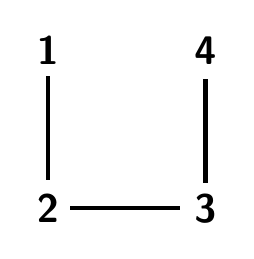
\begin{tikzpicture}[shorten >=1pt, auto, node distance=3cm, ultra thick]
   \begin{scope}[every node/.style={font=\sffamily\Large\bfseries}]
    \node (v1) at (0,0) {1};
    \node (v2) at (0,-2) {2};
    \node (v3) at (2,-2) {3};
    \node (v4) at (2,0) {4};

   \end{scope}
   \begin{scope}[every edge/.style={draw=black,ultra thick}]
    \draw  (v1) edge node{} (v2);
    \draw  (v2) edge node{} (v3);
    \draw  (v3) edge node{} (v4);
   \end{scope}
\end{tikzpicture}
\end{figure}
$$G_1$$
\begin{figure}[H]
\centering
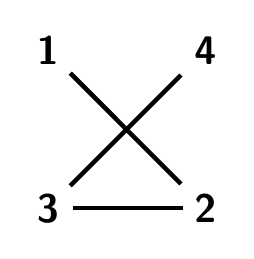
\begin{tikzpicture}[shorten >=1pt, auto, node distance=3cm, ultra thick]
   \begin{scope}[every node/.style={font=\sffamily\Large\bfseries}]
    \node (v1) at (0,0) {1};
    \node (v2) at (2,-2) {2};
    \node (v3) at (0,-2) {3};
    \node (v4) at (2,0) {4};

   \end{scope}
   \begin{scope}[every edge/.style={draw=black,ultra thick}]
    \draw  (v1) edge node{} (v2);
    \draw  (v2) edge node{} (v3);
    \draw  (v3) edge node{} (v4);
   \end{scope}
\end{tikzpicture}
\end{figure}
$$G_2$$
\begin{figure}[H]
\centering
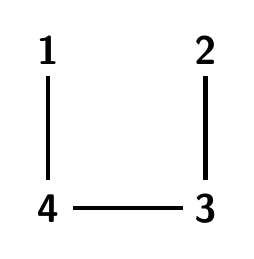
\begin{tikzpicture}[shorten >=1pt, auto, node distance=3cm, ultra thick]
   \begin{scope}[every node/.style={font=\sffamily\Large\bfseries}]
    \node (v1) at (0,0) {1};
    \node (v2) at (2,0) {2};
    \node (v3) at (2,-2) {3};
    \node (v4) at (0,-2) {4};

   \end{scope}
   \begin{scope}[every edge/.style={draw=black,ultra thick}]
    \draw  (v1) edge node{} (v4);
    \draw  (v2) edge node{} (v3);
    \draw  (v3) edge node{} (v4);
   \end{scope}
\end{tikzpicture}
\end{figure}
\end{multicols}
$$G=G_1\ \ G\neq G_2$$
\end{example*}

\begin{definition}[Graf dwudzielny]~ %%% <-  Note that space!
Graf $G$ nazywamy \underline{Grafem dwudzielnym} jeżeli zbiór $V$ można podzielić na dwa zbiory $V=X\cup Y$ tak, żeby każda krawędź miała jeden koniec w $X$ a drugi w $Y$ 
\end{definition}
\begin{tikzpicture}[
  every node/.style={on grid},
  setA/.style={fill=blue,circle,inner sep=2pt},
  setC/.style={fill=red,rectangle,inner sep=2pt},
  every fit/.style={draw,fill=blue!15,ellipse,text width=25pt},
  >=latex
]

% set A
\node[setA,label=left:] (a) {};
\node [setA,below = of a] (b) {};
\node [setA,below = of b] (c) {};
\node [setA,below = of c] (d) {};
\node [setA,below = of d] (e) {};
\node[above=of a,anchor=south] {$X$};

% set C
\node[setC,right = 3cm of a] (m) {};
\node[setC,below = of m] (n) {};
\node[setC,below = of n] (p) {};
\node[above=of m,anchor=south] {$Y$};

% the arrows
\draw[-] (a) -- node[] {} (m);
\draw[-] (b) -- node[] {} (m);
\draw[-] (c) -- node[] {} (p);
\draw[-] (e) -- node[] {} (n);

% the boxes around the sets
\begin{pgfonlayer}{background}
\node[fit= (a)  (e) ] {};
\node[fit= (m) (p)] {};
\end{pgfonlayer}
\end{tikzpicture}

\begin{example*}~ %%% <-  Note that space!
\begin{enumerate}
\item Graf pełny $K_n$
$$K_n\{[n]\footnotemark ,\{\{i,j\}, 1\leq i< j\leq n\}\}$$\footnotetext{$[n]=\{1,2,...,n\}$}

\item Pełny graf dwudzielny $K_{n,m}$
\begin{align*}
V=X\cup Y & |X|=n &|Y|=m\\
|E|=n*m
\end{align*}
\begin{multicols}{2}[$$K_{3,3}$$]
\begin{figure}[H]
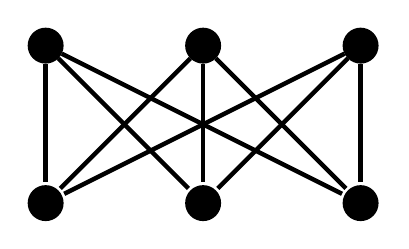
\begin{tikzpicture}[shorten >=1pt, auto, node distance=3cm, ultra thick,main node/.style={circle,fill=black,draw,minimum size=.4cm,inner sep=0pt]}]
\begin{scope}[every node/.style={font=\sffamily\Large\bfseries}]
\node[main node] (v1) at (0,0) {};
\node[main node] (v2) at (2,0) {};
\node[main node] (v3) at (4,0) {};
\node[main node] (v4) at (0,-2) {};
\node[main node] (v5) at (2,-2) {};
\node[main node] (v6) at (4,-2) {};
\end{scope}
\begin{scope}[every edge/.style={draw=black,ultra thick}]
\draw  (v1) edge node{} (v4);
\draw  (v1) edge node{} (v5);
\draw  (v1) edge node{} (v6);
\draw  (v2) edge node{} (v4);
\draw  (v2) edge node{} (v5);
\draw  (v2) edge node{} (v6);
\draw  (v3) edge node{} (v4);
\draw  (v3) edge node{} (v5);
\draw  (v3) edge node{} (v6);
\end{scope}
\end{tikzpicture}
\end{figure}
\begin{figure}[H]
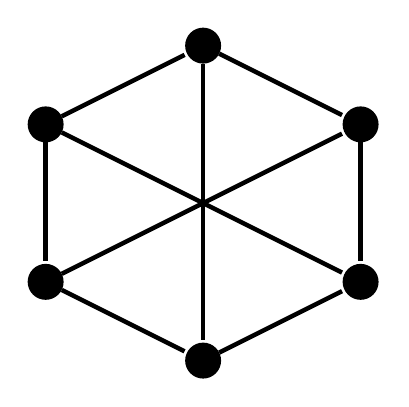
\begin{tikzpicture}[shorten >=1pt, auto, node distance=3cm, ultra thick,main node/.style={circle,draw,fill=black,minimum size=.4cm,inner sep=0pt]}]%
\begin{scope}[every node/.style={font=\sffamily\Large\bfseries}]
\node[main node] (v1) at (0,0) {};
\node[main node] (v2) at (0,-2) {};
\node[main node] (v3) at (2,1) {};
\node[main node] (v4) at (4,0) {};
\node[main node] (v5) at (4,-2) {};
\node[main node] (v6) at (2,-3) {};
\end{scope}
\begin{scope}[every edge/.style={draw=black,ultra thick}]
\draw  (v1) edge node{} (v2);
\draw  (v1) edge node{} (v3);
\draw  (v1) edge node{} (v5);
\draw  (v2) edge node{} (v4);
\draw  (v6) edge node{} (v5);
\draw  (v2) edge node{} (v6);
\draw  (v3) edge node{} (v4);
\draw  (v4) edge node{} (v5);
\draw  (v3) edge node{} (v6);
\end{scope}
\end{tikzpicture}
\end{figure}
\end{multicols}

\item $C_n$ $\rightarrow$ Cykl na $n$ wierzchołkach
\begin{figure}[H]
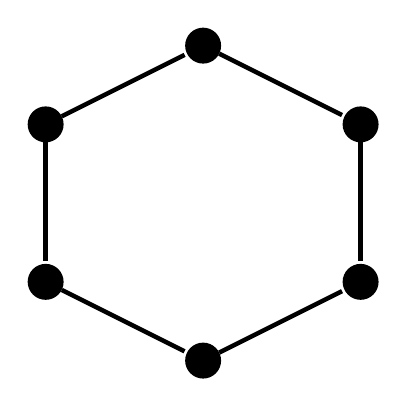
\begin{tikzpicture}[shorten >=1pt, auto, node distance=3cm, ultra thick,main node/.style={circle,draw,fill=black,minimum size=.4cm,inner sep=0pt]}]%
\begin{scope}[every node/.style={font=\sffamily\Large\bfseries}]
\node[main node] (v1) at (0,0) {};
\node[main node] (v2) at (0,-2) {};
\node[main node] (v3) at (2,1) {};
\node[main node] (v4) at (4,0) {};
\node[main node] (v5) at (4,-2) {};
\node[main node] (v6) at (2,-3) {};
\end{scope}
\begin{scope}[every edge/.style={draw=black,ultra thick}]
\draw  (v1) edge node{} (v2);
\draw  (v1) edge node{} (v3);
%\draw  (v2) edge node{} (v4);
\draw  (v6) edge node{} (v5);
\draw  (v2) edge node{} (v6);
\draw  (v3) edge node{} (v4);
\draw  (v4) edge node{} (v5);
%\draw  (v3) edge node{} (v6);
\end{scope}
\end{tikzpicture}
\end{figure}

\item $P_n$ $\rightarrow$ Ścieżka na $n$ wierzchołkach
\begin{figure}[H]
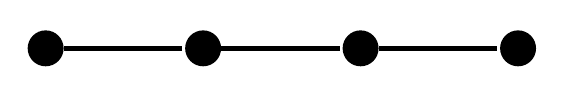
\begin{tikzpicture}[shorten >=1pt, auto, node distance=3cm, ultra thick,main node/.style={circle,draw,fill=black,minimum size=.4cm,inner sep=0pt]}]%
\begin{scope}[every node/.style={font=\sffamily\Large\bfseries}]
\node[main node] (v1) at (0,0) {};
\node[main node] (v2) at (2,0) {};
\node[main node] (v3) at (4,0) {};
\node[main node] (v4) at (6,0) {};
\end{scope}
\begin{scope}[every edge/.style={draw=black,ultra thick}]
\draw  (v1) edge node{} (v2);
\draw  (v2) edge node{} (v3);
\draw  (v3) edge node{} (v4);
\end{scope}
\end{tikzpicture}
\end{figure}
\end{enumerate}
\end{example*}

\begin{fact}~ %%% <-  Note that space!
\begin{itemize}
\item Ścieżka jest grafem dwudzielnym
\item Cykl jest grafem dwudzielnym, jeżeli liczba elementów ($n$) jest parzysta
\end{itemize}
\end{fact}

\begin{definition}[Skojarzenie]~ %%% <-  Note that space!
\underline{Skojarzeniem} $M$ w grafie $G=(V,E)$ nazywamy taki podzbiór rozłączny krawędzi grafu $G$, gdy nie zawiera pętli i żadne dwie krawędzie z $M$ nie są przyległe. Dwa końce krawędzi z $M$ są skojarzone prze $M$
\begin{figure}[H]
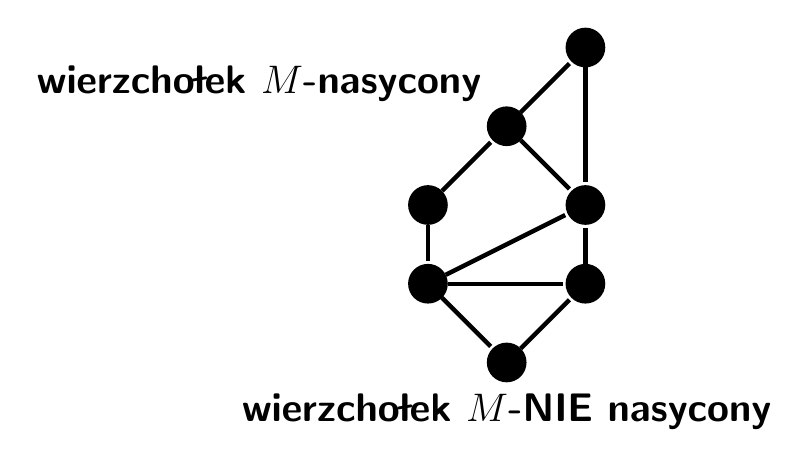
\begin{tikzpicture}[shorten >=1pt, auto, node distance=3cm, ultra thick,main node/.style={circle,draw,minimum size=.4cm,fill=black,inner sep=0pt]}]%fill=black,
\begin{scope}[every node/.style={font=\sffamily\Large\bfseries}]
\node[main node] (v1) at (0,0) {1};
\node[main node, label=above left:wierzchołek $M$-nasycony] (v2) at (1,1) {2};
\node[main node] (v3) at (2,2) {3};
\node[main node] (v4) at (2,0) {4};
\node[main node] (v5) at (0,-1) {5};
\node[main node, label=below:wierzchołek $M$-NIE nasycony] (v6) at (1,-2) {6};
\node[main node] (v7) at (2,-1) {7};
\end{scope}
\begin{scope}[every edge/.style={draw=black,ultra thick}]
\draw  (v1) edge node{} (v2);
\draw  (v1) edge node{} (v5);
\draw  (v2) edge node{} (v3);
\draw  (v2) edge node{} (v4);
\draw  (v3) edge node{} (v4);
\draw  (v5) edge node{} (v4);
\draw  (v5) edge node{} (v7);
\draw  (v5) edge node{} (v6);
\draw  (v6) edge node{} (v7);
\draw  (v7) edge node{} (v4);
\end{scope}
\end{tikzpicture}
\end{figure}
\end{definition}

\begin{definition}[Skojarzenie nasycone]~ %%% <-  Note that space!
Skojarzenie $M$ nazywamy doskonałym, gdy nasyca wszystkie wierzchołki.
\end{definition}

\begin{problem*}~ %%% <-  Note that space!
Kiedy graf dwudzielny $G=(X\cup Y, E)$ posiada skojarzenie nasycające wszystkie wierzchołki z $X$?
\begin{figure}[H]
\begin{tikzpicture}[
  every node/.style={on grid},
  setA/.style={fill=blue,circle,inner sep=2pt},
  setC/.style={fill=red,rectangle,inner sep=2pt},
  every fit/.style={draw,fill=blue!15,ellipse,text width=25pt},
  >=latex
]

% set A
\node[setA,label=left:] (a) {};
\node [setA,below = of a] (b) {};
\node [setA,below = of b] (c) {};
\node [setA,below = of c] (d) {};
\node[above=of a,anchor=south] {$X$};

% set C
\node[setC,right = 3cm of a] (m) {};
\node[setC,below = of m] (n) {};
\node[setC,below = of n] (p) {};
\node[setC,below = of p] (q) {};
\node[setC,below = of q] (r) {};
\node[above=of m,anchor=south] {$Y$};

% the arrows
\draw[-] (a) -- node[] {} (m);
\draw[-] (a) -- node[] {} (n);
\draw[-] (b) -- node[] {} (n);
\draw[-] (c) -- node[] {} (m);
\draw[-] (d) -- node[] {} (p);
\draw[-] (d) -- node[] {} (q);
\draw[-] (d) -- node[] {} (r);

% the boxes around the sets
\begin{pgfonlayer}{background}
\node[fit= (a)  (c) ] {};
\node[fit= (m) (n)] {};
\end{pgfonlayer}
\end{tikzpicture}
\end{figure}
\begin{align*}
&N(S)=\left \{ x:\exists _{y\in S}:x,y\in E \right \}\\
&|N(S)|< |S|
\end{align*}
\end{problem*}

\begin{theorem}[Hall]\label{the:Hall}
Graf dwudzielny $G=(X\cup Y,E)$ ma skojarzenie nasycające każdy wierzchołek $X$ wtedy i tylko wtedy, gdy spełniony jest warunek:
$$\forall _{S\subseteq X}|N(S)|\geq |S|$$
\end{theorem}
\begin{proof}~ %%% <-  Note that space!
\begin{description}
\item[$\Rightarrow$] Oczywisty
\item[$\Leftarrow$] Nie jest specjalnie trudy
\end{description}
\end{proof}
\begin{fact*}~ %%% <-  Note that space!
Istnieje szybki (działający w czasie wielomianowym) algorytm, który znajduje skojarzenie nasycające $X$ albo zbiór $S$, który nie spełnia warunku $(\star )$.
\end{fact*}

\begin{problem*}~ %%% <-  Note that space!
Czy dany graf zawiera skojarzenia doskonałe?
\end{problem*}
$$G(V,E),\ \ S\subseteq V$$
$o(G\setminus S)\rightarrow$ liczba składowych nieparzystych w grafie otrzymanych z $G$ przez ,,wyrzucenie'' wierzchołków z $S$ i wszystkich krawędzi o końcach w $S$

\begin{definition}[Składowa grafu]~ %%% <-  Note that space!
Składowa grafu to część grafu w której z każdej części można dostać się do całości grafu.
\end{definition}
\begin{multicols}{2}
\begin{figure}[H]
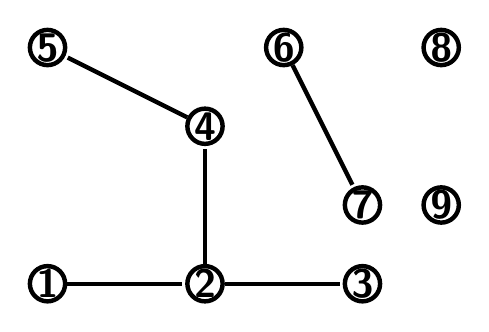
\begin{tikzpicture}[shorten >=1pt, auto, node distance=3cm, ultra thick,main node/.style={circle,draw,minimum size=.4cm,inner sep=0pt]}]%fill=black,
\begin{scope}[every node/.style={font=\sffamily\Large\bfseries}]
\node[main node] (v1) at (0,0) {1};
\node[main node] (v2) at (2,0) {2};
\node[main node] (v3) at (4,0) {3};
\node[main node] (v4) at (2,2) {4};
\node[main node] (v5) at (0,3) {5};
\node[main node] (v6) at (3,3) {6};
\node[main node] (v7) at (4,1) {7};
\node[main node] (v8) at (5,3) {8};
\node[main node] (v9) at (5,1) {9};
\end{scope}
\begin{scope}[every edge/.style={draw=black,ultra thick}]
\draw  (v1) edge node{} (v2);
\draw  (v2) edge node{} (v3);
\draw  (v2) edge node{} (v4);
\draw  (v4) edge node{} (v5);
\draw  (v6) edge node{} (v7);
\end{scope}
\end{tikzpicture}
\caption*{$G_1$}
\end{figure}
$G_1$ Ma 4 składowe:\\
$\{\{1,2,3,4,5\}, \{6,7\},\{8\},\{9\}\}$
\begin{figure}[H]
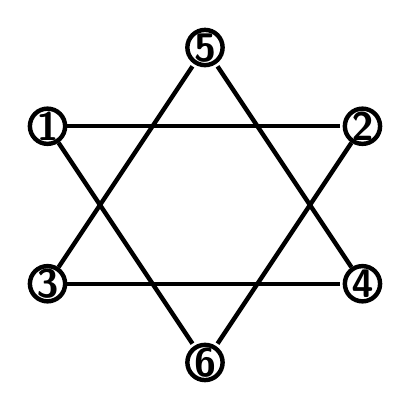
\begin{tikzpicture}[shorten >=1pt, auto, node distance=3cm, ultra thick,main node/.style={circle,draw,minimum size=.4cm,inner sep=0pt]}]%fill=black,
\begin{scope}[every node/.style={font=\sffamily\Large\bfseries}]
\node[main node] (v3) at (0,0) {1};
\node[main node] (v4) at (4,0) {2};
\node[main node] (v1) at (0,-2) {3};
\node[main node] (v2) at (4,-2) {4};
\node[main node] (v5) at (2,1) {5};
\node[main node] (v6) at (2,-3) {6};
\end{scope}
%Jahwe?
\begin{scope}[every edge/.style={draw=black,ultra thick}]
\draw  (v1) edge node{} (v2);
\draw  (v1) edge node{} (v5);
\draw  (v2) edge node{} (v5);
\draw  (v3) edge node{} (v4);
\draw  (v3) edge node{} (v6);
\draw  (v4) edge node{} (v6);
\end{scope}
\end{tikzpicture}
\caption*{$G_2$}
\end{figure}
$G_2$ Ma 2 składowe: $\{\{1,2,6\},\{3,4,5\}\}$
\begin{figure}[H]
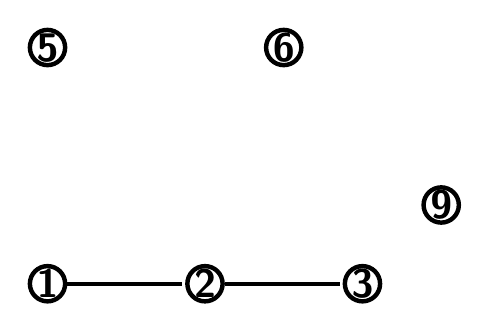
\begin{tikzpicture}[shorten >=1pt, auto, node distance=3cm, ultra thick,main node/.style={circle,draw,minimum size=.4cm,inner sep=0pt]}]%fill=black,
\begin{scope}[every node/.style={font=\sffamily\Large\bfseries}]
\node[main node] (v1) at (0,0) {1};
\node[main node] (v2) at (2,0) {2};
\node[main node] (v3) at (4,0) {3};
\node[main node] (v5) at (0,3) {5};
\node[main node] (v6) at (3,3) {6};
\node[main node] (v9) at (5,1) {9};
\end{scope}
\begin{scope}[every edge/.style={draw=black,ultra thick}]
\draw  (v1) edge node{} (v2);
\draw  (v2) edge node{} (v3);
\end{scope}
\end{tikzpicture}
\caption*{$G\setminus S$}
\end{figure}
$S=\{4,7,8\}$ $\Rightarrow$ $o(G\setminus S)=4$
\end{multicols}

\begin{theorem}[Tutte '47]\label{the:Tutte}~ %%% <-  Note that space!
Graf $G$ ma skojarzenie doskonałe wtedy i tylko wtedy, gdy
$$\forall _{S\subseteq V}o(G\setminus S) \leq |S|$$
\end{theorem}
\begin{proof}~ %%% <-  Note that space!
\begin{figure}[H]
\centering
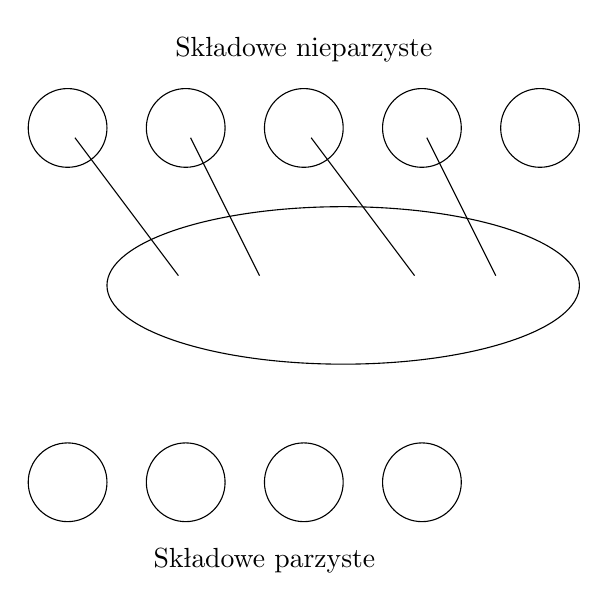
\begin{tikzpicture}
\draw  (0,0.5) ellipse (3 and 1);
\draw  (-3.5,2.5) node (v1) {} ellipse (0.5 and 0.5);
\draw  (-2,2.5) node (v3) {} ellipse (0.5 and 0.5);
\draw  (-0.5,2.5) node (v5) {} ellipse (0.5 and 0.5);
\draw  (1,2.5) node (v7) {} ellipse (0.5 and 0.5);
\draw  (2.5,2.5) ellipse (0.5 and 0.5);
\node (v2) at (-2,0.5) {};
\node (v4) at (-1,0.5) {};
\node (v6) at (1,0.5) {};
\node (v8) at (2,0.5) {};
\draw  (v1) edge (v2);
\draw  (v3) edge (v4);
\draw  (v5) edge (v6);
\draw  (v7) edge (v8);
\draw  (-3.5,-2) ellipse (0.5 and 0.5);
\draw  (-2,-2) ellipse (0.5 and 0.5);
\draw  (-0.5,-2) ellipse (0.5 and 0.5);
\draw  (1,-2) ellipse (0.5 and 0.5);
\node at (-0.5,3.5) {Składowe nieparzyste};
\node at (-1,-3) {Składowe parzyste};
\end{tikzpicture}
\end{figure}
\end{proof}

\begin{theorem}~ %%% <-  Note that space!
Graf jest dwudzielny wtedy i tlko wtedy, gdy nie zawiera cykli nieparzystych
\end{theorem}
\begin{proof}~ %%% <-  Note that space!
\begin{description}
\item[$\Rightarrow$] Oczywisty
\item[$\Leftarrow$] Jeżeli nie da się podzielić to zawiera cykle nieparzyste
\end{description}
\end{proof}
\subsection{Dygresja na temat złożoności}
\textbf{Pytanie:}
\begin{enumerate}
\item Które problemy można szybko rozwiązać (i co to znaczy szybko)?
\item Czy istnieje dla danego problemu szybki algorytm?
\end{enumerate}
\begin{fact*}[Endmonds '63]~ %%% <-  Note that space!
Istnieje wielomianowy algorytm znajdujący skojarzenia doskonałe
\end{fact*}
\begin{description}
\item[P] daje odpowiedź w czasie wielomianowym
\item[NP] klasa problemów takich, że odpowiedź $\mathsf{TAK}$ można zweryfikować w czasie wielomianowym. 
\end{description}
\begin{example*}~ %%% <-  Note that space!
Problem czy graf ma skojarzenie doskonałe? $\Rightarrow$ należy do \textbf{NP}

Twierdzenie Tutte'a mówi, że ten problem należy do klasy \textbf{coNP}
\end{example*}
\begin{problem*}~ %%% <-  Note that space!
Czy liczba $p$ jest pierwsza? $\Rightarrow $ \textbf{coNP} $\land$ \textbf{NP}
\end{problem*}

%--------------------------------------------------